\documentclass[AMA,twocolumn]{USG}
\usepackage{xcolor}
\usetikzlibrary{positioning, shapes.geometric, arrows.meta}
\usepackage{minted}
\usemintedstyle{trac}
\setminted{fontsize=\footnotesize, breaklines=true, breakanywhere=true}

\definecolor{LightGray}{gray}{0.9}
\linespread{1.5}

\articletype{Undertale in Extremis: Simulador de Batalhas em Risc-V}

\begin{document}

\title{Trabalho de Organização de Computadores\thanks{Código fonte disponível em: \url{https://github.com/lyszt/undertale-in-extremis\_core}}}

\author[1]{João Luís Almeida Santos}

\address[1]{\orgname{Universidade Federal da Fronteira Sul,}%
\orgaddress{\city{Chapecó}, \state{Santa Catarina}, \country{Brasil}}}

\maketitle

\section{Introdução}
\begin{figure}[h]
\centering

\includegraphics[width=\linewidth]{images/jogo.png}
\caption{Interface do simulador de batalhas no modo de observação.}\label{fig:jogo}
\end{figure}

O presente projeto documenta a tentativa de criar um simulador de batalhas de RPG, no estilo Pokémon (Figura~\ref{fig:jogo}),
dentro do ambiente RISC-V, utilizando o RARS como ferramenta de simulação. A ISA utilizada é a
RISC-V RV32IM, isto é, um conjunto de instruções que contempla apenas operações com inteiros,
além de instruções de multiplicação e divisão.
\\\\
O projeto, denominado \textit{Undertale in Extremis}, foi desenvolvido como proposta alternativa 
às opções listadas na comanda, com autorização do professor.
 O sistema simula batalhas entre dois bots autônomos que se enfrentam em 
 turnos até que um deles seja eliminado. Cada bot recebe uma estratégia e age por conta própria, 
 escolhendo a cada turno entre seis ações: ataque, defesa, Absolute Grit, Soul Suck, Final Execution e Mirror Shield.
 Ambos os bots iniciam com 100 pontos de vida (HP) e 100 de mana (MP), sendo o MP regenerado em +2 por turno.
\\\\
\vspace{4pt}\noindent\captionof{table}{Ações disponíveis por turno}
{\renewcommand{\arraystretch}{1.5}
\begin{tabular}{p{1.8cm}p{4.5cm}p{1.2cm}}
\hline
\textbf{Ação} & \textbf{Efeito} & \textbf{Custo} \\
\hline
Ataque         & 1d20: erro $<$10, hit $\geq$10, dúplica o dano em 20. & 0 MP \\
Defesa         & Bloqueia o próximo ataque. Contra-ataca quando crítico. & 0 MP \\
Absolute Grit  & Garante um crítico. & 20 MP \\
Soul Suck      & 1--12 de auto-dano; ganha 4$\times$ em MP. & 0 MP \\
Final Execution & 800\% de dano. Falha se alvo $>$50\% HP. & 150 MP \\
Mirror Shield  & Reflete o próximo ataque recebido. & 30 MP \\
\hline
\end{tabular}}
\vspace{4pt}


O ataque realiza uma verificação 1d20: abaixo de 10 erra, acima acerta, e no 20 resulta em crítico com dano dobrado.
A defesa bloqueia o próximo ataque recebido, podendo ripostar em um crítico.
A Absolute Grit garante um crítico ao custo de 20 MP.
A Soul Suck causa 1--12 de dano ao próprio bot, drenando igual MP do inimigo e ganhando 4$\times$ esse valor, podendo ultrapassar o limite de 100 MP.
A Final Execution causa 800\% de dano ao custo de 150 MP, mas falha se o alvo estiver acima de 50\% de HP.
O Mirror Shield reflete o próximo ataque recebido de volta ao atacante, ao custo de 30 MP.

\vspace{4pt}\noindent\captionof{table}{Atributos iniciais de cada bot}
{\renewcommand{\arraystretch}{1.5}
\begin{tabular}{ll}
\hline
\textbf{Atributo} & \textbf{Valor} \\
\hline
HP & 100 \\
MP & 100 \\
Regeneração de MP & +2 por turno \\
\hline
\end{tabular}}
\vspace{4pt}



\vspace{4pt}\noindent\captionof{table}{Estratégias dos bots}
{\renewcommand{\arraystretch}{1.5}
\begin{tabular}{p{1.2cm}p{1.4cm}p{4.5cm}}
\hline
\textbf{Bot} & \textbf{Estratégia} & \textbf{Comportamento} \\
\hline
Flowey & Aleatório  & Escolhe uma das seis ações por RNG a cada turno, sem avaliar estado algum. \\
Chara  & Inteligente & Acumula MP via Soul Suck até atingir 150 MP, reduz o inimigo abaixo de 50\% de HP com Absolute Grit e então dispara a Final Execution. \\
Toby   & Troll    & Monitora o próprio HP e o MP do inimigo. Se estiver abaixo de 50 HP e o inimigo tiver $\geq$150 MP, levanta o Mirror Shield para refletir a Final Execution. Fora dessa janela, mistura ataques e Soul Suck, e executa o inimigo quando as condições permitem. \\
\hline
\end{tabular}}
\vspace{4pt}


\section{Desafios e Soluções}

\subsection{Fluxo do Jogo}

O simulador segue um loop de turnos fixo. A cada turno, o bot ativo toma uma decisão com base na sua estratégia, executa a ação, os efeitos são aplicados, o MP regenera e o escudo espelho é verificado. Ao fim, o jogo checa se algum bot morreu. Se não, troca o turno e repete.

\begin{figure*}[t]
\centering
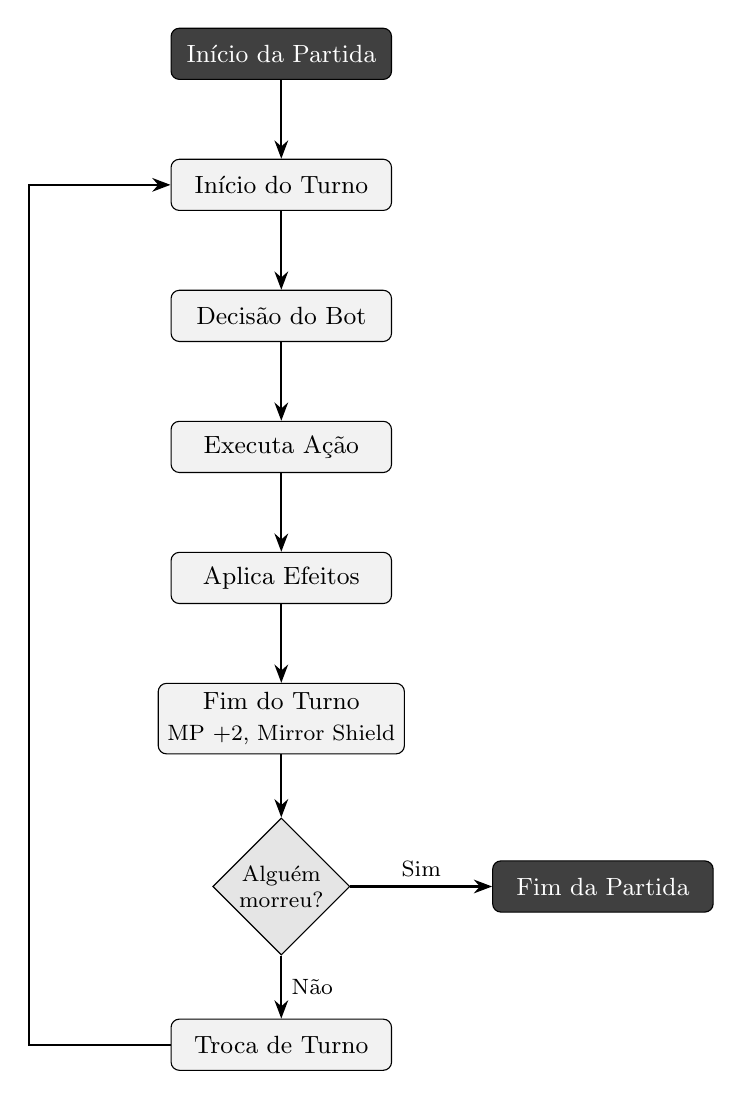
\begin{tikzpicture}[
  node distance=1cm and 1.8cm,
  state/.style={rectangle, rounded corners=3pt, draw, fill=gray!10, minimum width=2.8cm, minimum height=0.65cm, font=\small, align=center},
  terminal/.style={rectangle, rounded corners=3pt, draw, fill=black!75, text=white, minimum width=2.8cm, minimum height=0.65cm, font=\small, align=center},
  dec/.style={diamond, draw, fill=gray!20, minimum width=1cm, minimum height=0.65cm, font=\footnotesize, align=center, inner sep=1pt},
  arr/.style={->, >=Stealth, thick}
]

\node[terminal] (start) {Início da Partida};
\node[state, below=of start] (turn) {Início do Turno};
\node[state, below=of turn] (decide) {Decisão do Bot};
\node[state, below=of decide] (action) {Executa Ação};
\node[state, below=of action] (effects) {Aplica Efeitos};
\node[state, below=of effects] (endturn) {Fim do Turno\\{\footnotesize MP +2, Mirror Shield}};
\node[dec, below=0.8cm of endturn] (dead) {Alguém\\morreu?};
\node[state, below=0.8cm of dead] (swap) {Troca de Turno};
\node[terminal, right=of dead] (end) {Fim da Partida};

\draw[arr] (start) -- (turn);
\draw[arr] (turn) -- (decide);
\draw[arr] (decide) -- (action);
\draw[arr] (action) -- (effects);
\draw[arr] (effects) -- (endturn);
\draw[arr] (endturn) -- (dead);
\draw[arr] (dead) -- node[right]{\footnotesize Não} (swap);
\draw[arr] (dead) -- node[above]{\footnotesize Sim} (end);
\draw[arr] (swap.west) -- ++(-1.8,0) |- (turn.west);

\end{tikzpicture}
\caption{Fluxo de estados do simulador por turno.}
\label{fig:statemachine}
\end{figure*}

\subsection{Randomização}
Fazer um algoritmo que gerasse números realmente aleatórios foi desafiante. E para esse projeto, eu tive que
misturas alguns métodos. A base principal foi o Xorshift, inventado por Marsaglia em 2003 \cite{marsaglia2003xorshift}, publicado no
Journal of Statistical Software. 
Em seu artigo, Marsaglia descreve:
\begin{tcolorbox}[colback=gray!8, colframe=gray!40, boxrule=0.4pt, arc=2pt, left=4pt, right=4pt, top=4pt, bottom=4pt]
\normalsize\itshape
A xorshift random number generator (xorshift RNG) produces a sequence of $2^{32}-1$ integers $x$, or a sequence of $2^{64}-1$ pairs $x,y$, or a sequence of $2^{96}-1$ triples $x,y,z$, etc., by means of repeated use of a simple computer construction: exclusive-or (xor) a computer word with a shifted version of itself. In C, the basic operation is \texttt{y\^{}(y<<a)} for shifts left, \texttt{y\^{}(y>>a)} for shifts right. (In Fortran, a single form, \texttt{ieor(y,ishft(y,a))} will produce the desired result, with negative \texttt{a} for shifts right, nonnegative for shifts left.) Combining such xorshift operations for various shifts and arguments provides extremely fast and simple RNGs that seem to do well on tests of randomness. To give an idea of the power and effectiveness of xorshift operations, here is the essential part of a C procedure that, with only three xorshift operations per call, will provide $2^{128}-1$ random 32-bit integers, given four random seeds $x,y,z,w$: \cite{marsaglia2003xorshift}
\end{tcolorbox}

Em termos simples, o algoritmo pega um número aleatório, que é chamado de seed,
faz três operações de XOR com versões deslocadas de si mesmo, e 
o resultado é o próximo número da sequência. A seed é atualizada 
a cada chamada. No entanto, havia um problema. A seed colocada no .data era sempre a mesma, então o algoritmo
de randomização era na verdade, nada aleatório. Por isso, foi necessário utilizar a chamada de sistema de 
número 30 para multiplicar a seed pelos milisegundos do horário atual. No caso do número estourar, isso
é tranquilo, pois o overflow simplesmente descarta os bits mais altos. O 	
exttt{remu} é usado por dois motivos para limitar o resultado ao range desejado via módulo
e por ser a versão sem sinal da instrução, garantindo que o resultado nunca seja negativo,
já que o xorshift pode produzir valores negativos.

\begin{minted}{asm}
randomizer:
  mv      s0, a0            # salva o range maximo
  la      t3, seed
  lw      t0, 0(t3)         # carrega a semente atual

  slli    t1, t0, 13
  xor     t0, t0, t1        # xorshift esquerda 13
  srli    t1, t0, 17
  xor     t0, t0, t1        # xorshift direita 17
  slli    t1, t0, 5
  xor     t0, t0, t1        # xorshift esquerda 5

  remu    s1, t0, s0        # limita ao range; remu evita negativos
  addi    s1, s1, 1         # resultado em [1, range]

  li      a7, 30
  ecall                     # le o tempo atual do sistema
  mul     t5, a0, t0
  xor     t5, t5, t0        # mistura tempo com xorshift
  sw      t5, 0(t3)         # atualiza a semente

  mv      a1, s1
\end{minted}

\subsection{Gerenciamento de Stack}

O programa usa macros para abstrair e automatizar as operações necessárias de gerenciamento da stack
durante chamadas de função. Essa estratégia facilitou o desenvolvimento e reduziu a ocorrência de erros
relacionados ao gerenciamento da stack. O código apresentado corresponde a uma versão compatível apenas 
com o RARS, visto que, em outros \textit{assemblers}, utiliza-se a diretiva \texttt{.endm} 
em vez de \texttt{.end\_macro}. Aprendi essa técnica no último semestre de ORG.
\\\\

\begin{minted}{asm}
    .macro     startF
    addi       sp, sp, -20
    sw         ra, 16(sp)
    sw         s0, 12(sp)
    sw         s1, 8(sp)
    sw         s2, 4(sp)
    sw         s3, 0(sp)
    .end_macro

    .macro     endF
    lw         ra, 16(sp)
    lw         s0, 12(sp)
    lw         s1, 8(sp)
    lw         s2, 4(sp)
    lw         s3, 0(sp)
    addi       sp, sp, 20
    .end_macro

\end{minted}
Mesmo com os macros, o programa chegou a crashar durante o desenvolvimento. 
Algumas habilidades saíam da função via \texttt{j} para outro ponto do código 
em vez de retornar normalmente. Nesses casos, o \texttt{endF} nunca era executado: 
a stack crescia a cada uso da habilidade. A correção foi mover o \texttt{endF} para dentro de
\texttt{do\_attack\_crit\_no\_message}, que passa a desalocar a stack de quem saltou para ele.

\begin{minted}{asm}
do_absolute_grit:
  startF
  call calculate_damage
  j do_attack_crit_no_message  # endF nunca e chamado

# para consertar o problema foi necessário redefinir a função de crítico, e nessa versão alternativa,
# há um endF
\end{minted}

\subsection{Animação do modo de observação}
Outro desafio foi fazer as animações de forma bonita e em tempo real. Para esta parte, foi usada a Gemini Pro 3.0 para 
gerar os frames além do Ascii original, obtido de \cite{emojicombos_undertale}. Isso pelo fato de que todo personagem tem 5 frames de animação, e estes são definidos
dentro do .data. A forma de limpar a tela no terminal também foi algo que eu descobri pedindo para o Gemini Pro 3.0.

\begin{minted}{asm}
# quando o terminal lê esse byte, ele dá um espaçamento do tamanho atual da tela em que você está.
clear_screen: .byte 27, 91, 50, 74, 27, 91, 72, 0
# então na verdade ele não limpa o terminal, ele só dá um pulo pra baixo.
\end{minted}

Para o modo de simulação, a animação era muito lenta, pois utilizada a instrução 32 várias vezes para esperar 500 - 1000 milisegundos
para que as animações dessem a falsa impressão de serem fluídas. Sem esse wait, elas não podem ser vistas ou passam rápido demais. 
Por conta disso, o modo de benchmarking não tem animações, e portanto também não possui wait, e roda muito mais rápido. O modo é controlado por uma flag \texttt{modo\_play} no \texttt{.data}: quando ativa, o programa pula todo o bloco de renderização e vai direto para a próxima ação.

\begin{minted}{asm}
  la t0, modo_play
  lw t0, 0(t0)
  bnez t0, do_turn_action  # em benchmark pula a animacao
\end{minted}

Os bytes do \texttt{clear\_screen} correspondem à sequência de escape ANSI \texttt{ESC[2J} seguida de \texttt{ESC[H}: o primeiro apaga o conteúdo visível e o segundo move o cursor para o canto superior esquerdo. O efeito visual é o de limpeza, mas o histórico do terminal continua acessível com scroll.

\subsection{Decisões e Estratégias}

Cada turno, a função \texttt{decision} verifica a estratégia do bot ativo e salta para o ramo correspondente. O bot Troll é o mais complexo: ele lê o HP e MP de ambos os jogadores para decidir a ação. Se tiver MP suficiente e o inimigo estiver fraco, executa a Final Execution diretamente pelo ramo da estratégia Inteligente. Se o seu próprio HP estiver abaixo de 50 e o inimigo tiver 150 MP acumulados, levanta o Mirror Shield. Fora dessas condições, mistura ataque e Soul Suck aleatoriamente.

\begin{minted}{asm}
decision_troll_checks:
  li t6, 50
  ble t5, t6, decision_troll_check_enemy_mp
  j decision_troll_not_execute        # HP alto: nao precisa do escudo
decision_troll_check_enemy_mp:
  li t6, 150
  bge a3, t6, decision_troll_prepare_against_execute
  j decision_troll_not_execute        # inimigo sem mp: nao vai executar
decision_troll_prepare_against_execute:
  li a0, 6                            # Mirror Shield
  endF
  ret
decision_troll_not_execute:
  li a0, 6
  call randomizer
  li t6, 3
  bge a1, t6, decision_troll_attack
  j decision_troll_soul_suck
decision_troll_attack:
  li a0, 1  # Attack
  endF
  ret
decision_troll_soul_suck:
  li a0, 4  # Soul Suck
  endF
  ret
\end{minted}

\subsection{Habilidades}

O randomizador calculava o dano em \texttt{t1}, registrador temporário que não é preservado por \texttt{ecall}. No meio da função, um ecall para leitura do tempo atualizava a semente do gerador, corrompendo o valor em \texttt{t1}. O dano resultante virava negativo, e a subtração de HP funcionava como cura.

\begin{minted}{asm}
remu    t1, t0, s0  # resultado corrompido pelo ecall seguinte
addi    t1, t1, 1
\end{minted}

A correção foi mover o resultado para \texttt{s1}, que é preservado por chamadas de sistema.

Ao verificar o status do escudo, o código calculava o offset do array com \texttt{slli t2, t2, 4} em vez de \texttt{slli t2, t2, 2}. Cada elemento do array ocupa uma word (4 bytes), então o shift correto é de 2 bits. Com shift de 4, o offset era 4 vezes maior que o esperado, lendo uma posição de memória completamente errada e fazendo o escudo nunca ativar.

O primeiro problema era de lógica na decisão: sem um \texttt{j} explícito após a verificação de HP, o código caía diretamente na checagem de MP do inimigo independentemente da condição, fazendo o Toby levantar o escudo com frequência errada.

\begin{minted}{asm}
  ble t5, t6, decision_troll_check_enemy_mp
  # faltava: j decision_troll_not_execute
decision_troll_check_enemy_mp:
\end{minted}

O segundo era de design: fora da janela do escudo, Toby usava Soul Suck como ação padrão. Isso causava auto-dano constante sem benefício real contra Flowey, que nunca acumula MP. A correção foi trocar Soul Suck por uma mistura de ataque e defesa.
Houveram outros problemas documentados, só que alguns deles se mantiveram como features reais. A execução
não foi feita para causar 800\% de dano, foi pensada para apenas causar o dobro. Mas houve um erro de cálculo e 
uma junção de multiplicações, e, nesse caso, foi mantido o bug porque realmente era mais certeiro.
\section{Conclusão}

O projeto resultou em um simulador de batalhas funcional em assembly RISC-V, com três bots e um modo de benchmark que roda 10.000 partidas automaticamente.
Os resultados do benchmark foram contraintuitivos, conforme a Tabela~\ref{tab:winrates}. Normalmente, esperaria-se que os algoritmos mais 
planejados seriam mais eficazes, no entanto, o contrário ocorreu.

\vspace{4pt}\noindent
{\renewcommand{\arraystretch}{1.5}
\begin{tabular}{ll}
\hline
\textbf{Bot} & \textbf{Taxa de vitória} \\
\hline
Flowey & $\sim$52\% \\
Toby   & $\sim$29\% \\
Chara  & $\sim$17\% \\
\hline
\end{tabular}}\label{tab:winrates}
\vspace{4pt}

Flowey, o bot aleatório, ganhou a maioria das partidas. Chara, a mais elaborada, ficou em último. Com apenas seis ações e dano alto por turno, uma estratégia cuidadosa não tem vantagem real sobre o caos. O plano original incluía mais bots, mas balancear se mostrou difícil, e o espaço de ação era pequeno demais para que um quarto bot fizesse algo diferente dos três já existentes.

Na parte técnica, o projeto exigiu lidar com coisas que linguagens de alto nível escondem: stack manual, preservação de registradores e controle de fluxo via saltos. Os bugs foram difíceis de achar justamente por serem silenciosos, como o stack leak da Absolute Grit e o ataque que curava por corrupção de registrador.

\section{Utilização de IA}

Em conformidade com a observação da comanda, segue a declaração explícita dos trechos em que ferramentas de IA generativa foram utilizadas.

\subsection{Pesquisa de conceitos}
O algoritmo XORShift de Marsaglia foi descoberto a partir de uma consulta ao Gemini sobre geradores de números pseudoaleatórios eficientes para ambientes com recursos limitados. A ferramenta indicou o algoritmo e a referência original, que foi então consultada diretamente.

\subsection{Depuração}
Em casos onde o bug não era visível pela leitura do código, trechos do assembly foram submetidos ao Gemini para identificar possíveis causas. Foi o caso do ataque que curava, onde a corrupção do registrador \texttt{t1} pelo \texttt{ecall} não era óbvia.

\subsection{Revisão do relatório}
O texto do relatório passou por revisão gramatical assistida por IA.

\subsection{Geração de frames de animação}
Os frames ASCII dos personagens foram gerados com auxílio do Gemini Pro 3.0, a partir do ASCII original obtido em \cite{emojicombos_undertale}. O frame base de cada personagem foi editado manualmente para gerar as cinco variações de animação.

\section{Anexos}

\bibliographystyle{unsrt}
\bibliography{citacoes}

\end{document}
